\documentclass[12pt]{article}
\usepackage[a4paper, margin=1in]{geometry}
\usepackage{graphicx}
\usepackage{amsmath}
\usepackage{float}
\usepackage{caption}
\usepackage{subcaption}
\usepackage{hyperref}

\title{\textbf{Cam-scanner using OpenCV}}
\author{Niladri Ghosh \\
ID-B2430100 \\
Department of Computer Science}
\date{\today}

\begin{document}

\maketitle

\begin{abstract}
This report presents a computer vision-based document scanner using OpenCV. The pipeline involves detecting the boundary of a document from an image, applying a perspective transform, and enhancing the resulting image to resemble a scanned copy. This project simulates the core functionality of mobile scanning apps using simple yet effective image processing techniques.
\end{abstract}

\section{Introduction}
Scanning documents with a smartphone has become common practice. This project implements a custom scanner using Python and OpenCV. The main steps include:
\begin{itemize}
    \item Edge detection using Canny and contour approximation.
    \item Perspective transformation to "flatten" the image.
    \item Image enhancement using adaptive thresholding.
\end{itemize}

\section{Methodology}

\subsection{Step 1: Preprocessing}
The input image is resized and converted to grayscale for noise reduction and processing efficiency.

\begin{verbatim}
image = cv2.imread('doc.jpg')
image = cv2.resize(image, (1300,800))
gray = cv2.cvtColor(image, cv2.COLOR_BGR2GRAY)
blurred = cv2.GaussianBlur(gray, (5, 5), 0)
\end{verbatim}

\begin{figure}[H]
    \centering
    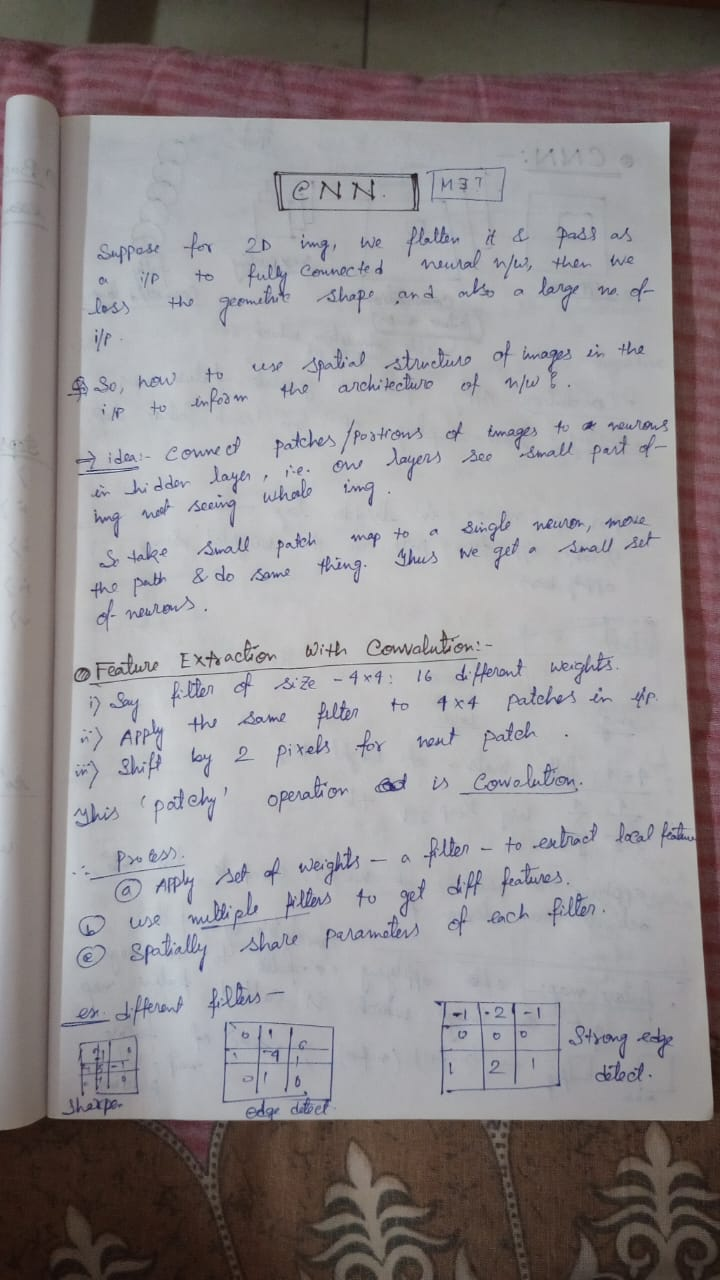
\includegraphics[width=0.7\textwidth]{doc.jpg}
    \caption{Original Input Image}
\end{figure}

\subsection{Step 2: Edge Detection and Contour Finding}
Canny edge detection is applied, and the largest contour approximated to four points is assumed to be the document boundary.

\begin{verbatim}
edged = cv2.Canny(blurred, 30, 50)
contours, _ = cv2.findContours(edged, cv2.RETR_LIST, cv2.CHAIN_APPROX_SIMPLE)
contours = sorted(contours, key=cv2.contourArea, reverse=True)[:5]
\end{verbatim}



\subsection{Step 3: Perspective Transform}
The detected contour is used to compute a perspective transform that warps the image, giving a top-down view.

\begin{verbatim}
warped = cv2.warpPerspective(image, matrix, (width, height))
\end{verbatim}


\subsection{Step 4: Image Enhancement}
To simulate the high-contrast appearance of scanned documents, adaptive thresholding is applied to the warped grayscale image.

\begin{verbatim}
final = cv2.adaptiveThreshold(
    gray_warped, 255, cv2.ADAPTIVE_THRESH_GAUSSIAN_C,
    cv2.THRESH_BINARY, 11, 2
)
\end{verbatim}



\section{Results}
The implemented pipeline successfully detects and transforms a document image into a top-down, high-contrast scan-like output. The adaptive thresholding helps improve readability and mimics the appearance of a physical scanner output.
\begin{figure}[H]
    \centering
    \begin{subfigure}[b]{0.45\textwidth}
        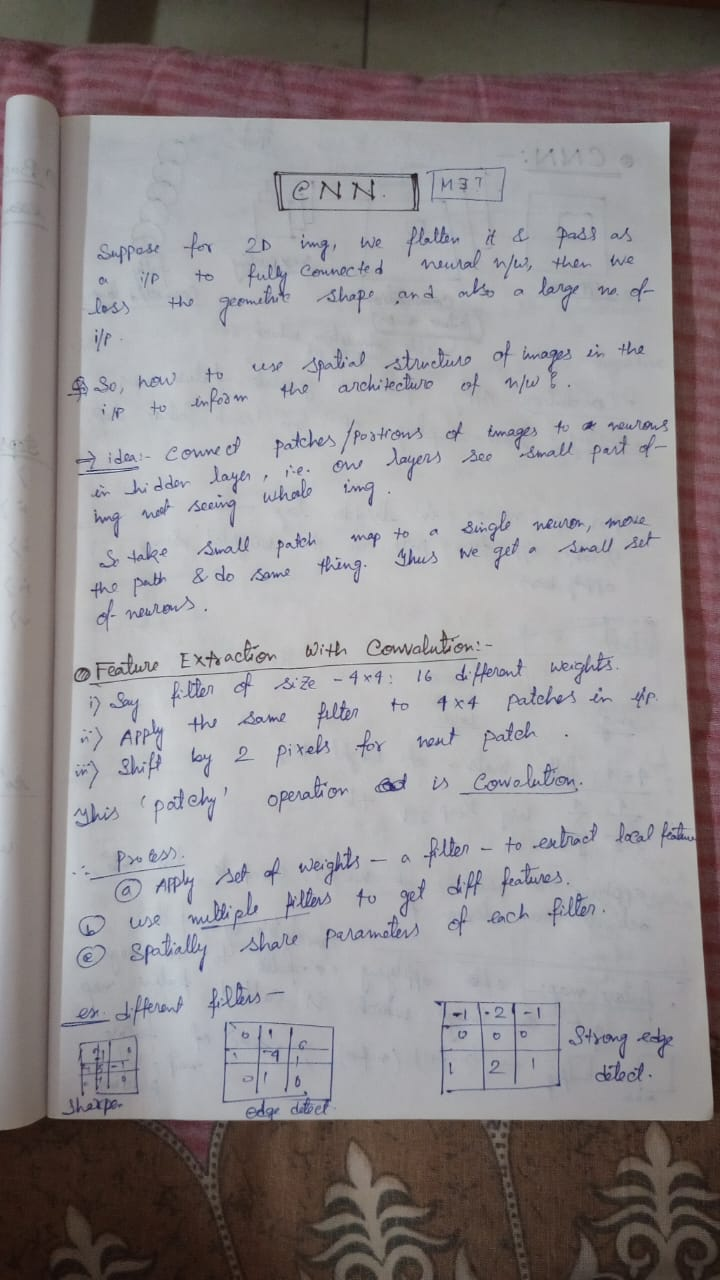
\includegraphics[width=\textwidth]{doc.jpg}
        \caption{Left Image}
    \end{subfigure}
    \hfill
    \begin{subfigure}[b]{0.45\textwidth}
        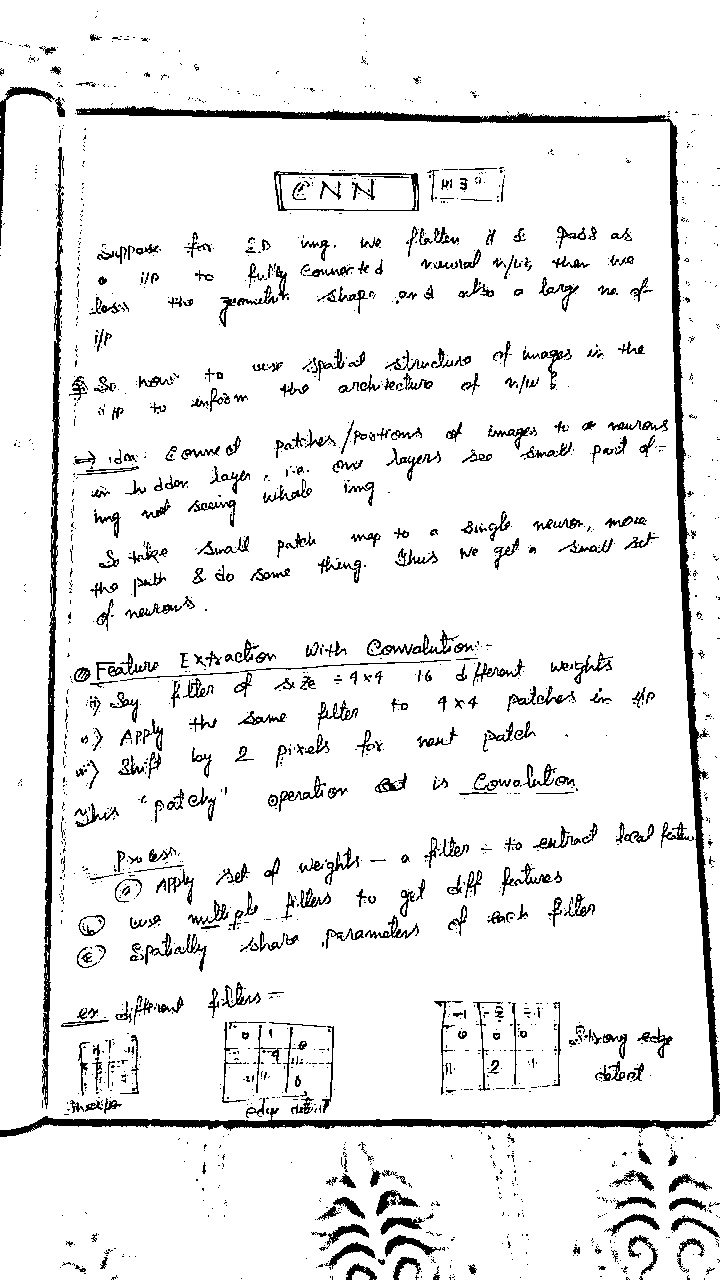
\includegraphics[width=\textwidth]{scanned_output.jpg}
        \caption{Right Image}
    \end{subfigure}
    \caption{Cam-scanner using OpenCV}
\end{figure}


\section{Conclusion}
This project demonstrates a simple but effective way to simulate a document scanner using OpenCV. The method is robust to perspective and lighting variations, making it suitable for practical use.

\section{Future Enhancements}
\begin{itemize}
    \item Add support for automatic document detection in a video stream.
    \item Implement text extraction using OCR (e.g., Tesseract).
    \item Improve lighting normalization for better scan quality.
\end{itemize}

\end{document}
